\section{Learning single-cell perturbation responses}
% TODO: finish
Popular approaches to model single-cell perturbation responses fall into three main camps, figure \ref{fig:arrows}.
The first takes a simple approach that ignores heterogeneity in response and models perturbations as linear shifts in data space, figure \ref{fig:arrows} left.
Cell typing approaches take this assumption, at least piece wise, and thus fail to capture any intra cell-type heterogeneity.
A popular approach is to model perturbation effects as a linear shift in some latent space that is then decoded with a non-linear function
These approaches include models like \textsc{scGen} \cite{lotfollahi2019} but many other models take similar approaches \cite{need}
While this approach is able to model heterogeneity, they need to implicitly solve a challenging disentanglement task \cite{locatello2018}, which, if not solved correctly, leads to aberrant behavior, figure \ref{fig:arrows} middle. 
In this work we opt to use a modern parameterization of an optimal transport coupling, figure \ref{fig:arrows} right.
Thanks to the mathematics of optimal transport, this allows us to predict treated states accurately by following a strict adherence to the control and treated distribution geometries.

\begin{figure}[ht]
  \begin{center}
    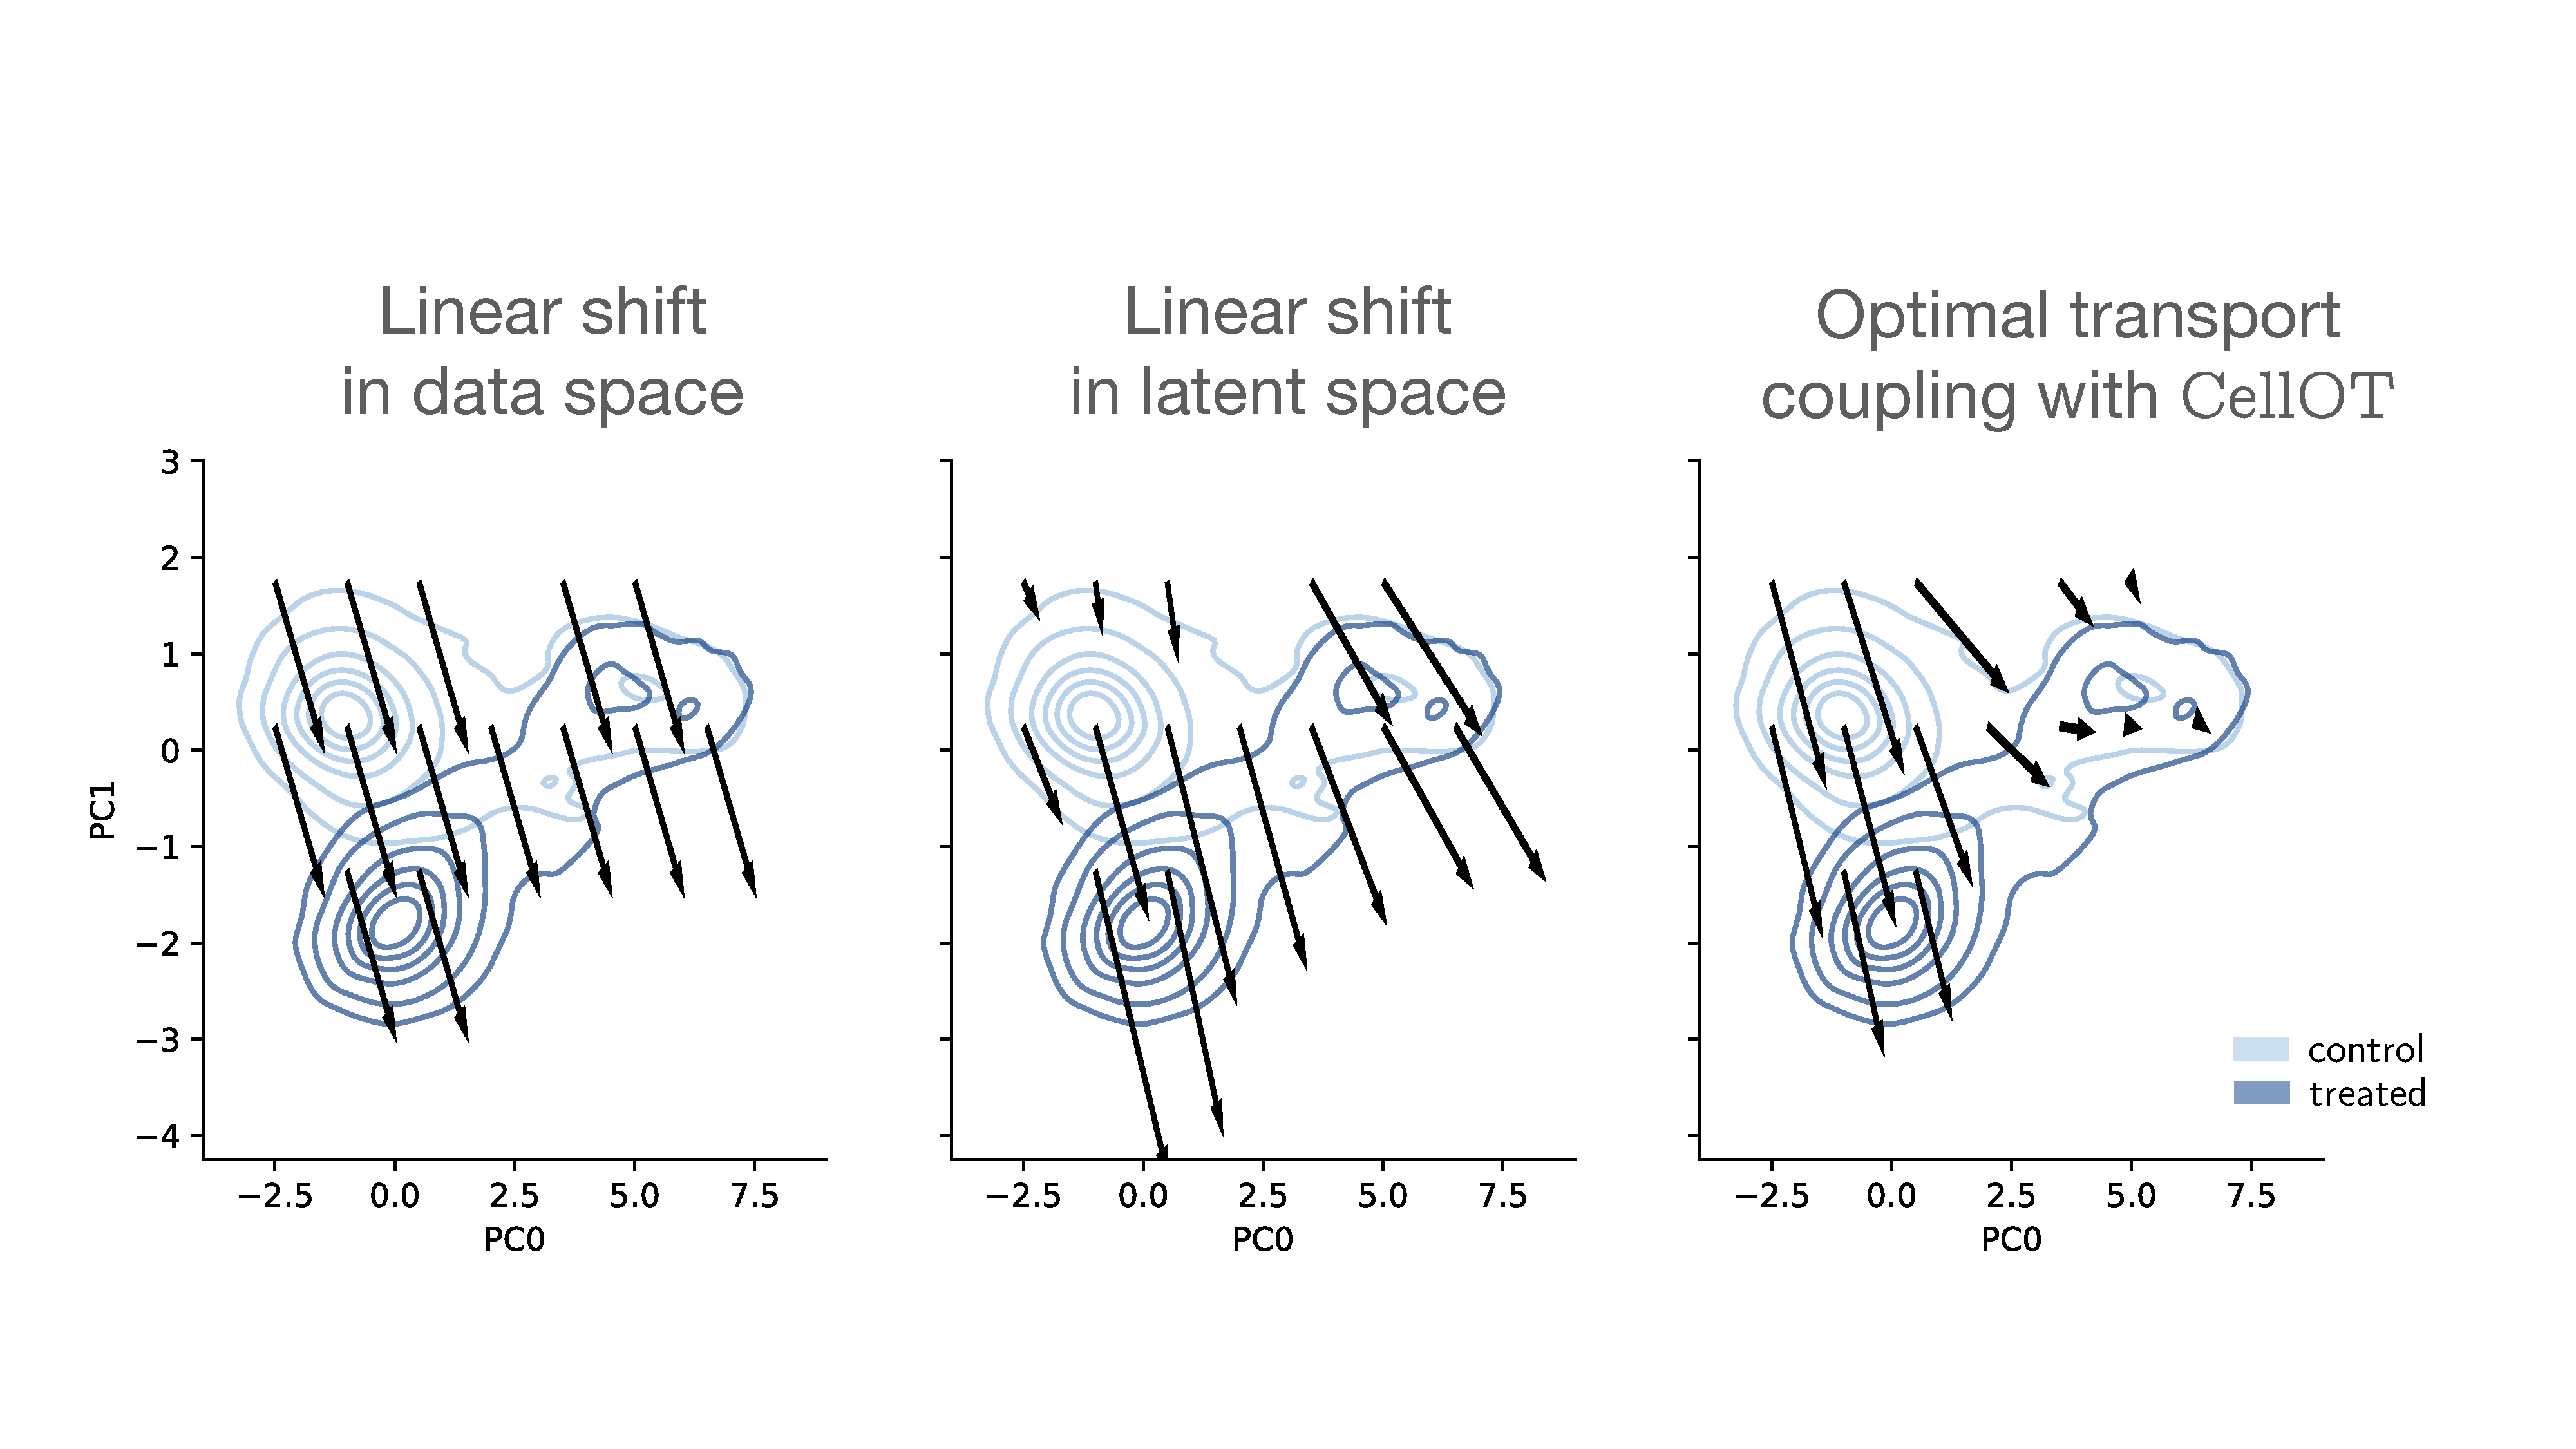
\includegraphics[width=0.95\textwidth]{figures/cellot-methods/arrow-cartoons.pdf}
  \end{center}
  \caption{Approaches to modeling single-cell perturbations. The control (light blue) and treated (dark blue) states are shown as a KDE plot. Arrows depict how each of the three approaches would predict responses at each location in feature space.}
  \label{fig:arrows}
\end{figure}


\subsection{Cell-type approaches}  % TODO: linear shifts in dataspace
Within one sample distinct cell types might exhibit very different responses toward a perturbation. This heterogeneity suggests modeling perturbation effects by first identifying different subpopulations and then predicting the response for each of those subpopulations individually. In the following, we introduce a method built upon that insight, which serves as a baseline in this study.

\paragraph{PopAlign}

\citet{chen2020dissecting} predict gene expression changes that occur in complex single-cell populations by identifying distinct subpopulations within that heterogeneous mixture for both the control $\rho_c$ and treated population $\rho_k$, and comparing as well as aligning those subpopulations in control and treated state through a probabilistic model.
To robustly identify those subpopulations, the data $X = \{ \mathbf{g}_i \}_{i=1}^k$ consisting of $n$-dimensional gene vectors $\mathbf{g}_i = (g_i^1, g_i^2, \dots, g_i^n)$ for each of the $k$ cells is embedded in a lower $m$-dimensional space using orthogonal nonnegative matrix factorization (oNMF) \citep{asteris2015orthogonal}, i.e., $Z = \{ \mathbf{c}_i \}_{i=1}^k$ with $\mathbf{c}_i = (c_i^1, c_i^2, \dots, c_i^m)$. oNMF is known to produce a meaningful set of features as the resulting representation is a superposition of largely disjoint features, here genes, shown to work well for clustering tasks.
This cluster structure then serves as the foundation to identify and represent subpopulations in both the control and subpopulation as $l$ independent Gaussian mixtures, i.e., $P(Z) = \sum_i^l w_i \mathcal{N}(Z; \mu_i, \Sigma_i)$ with weights $w_i$, centroids $\mu_i$, and covariance matrices $\Sigma_i$.
These parameters associated with each Gaussian density $(w_i, \mu_i, \Sigma_i)$ have a natural correspondence to the biological structure and semantics of those cell populations.
Lastly, to understand the perturbation response of each subpopulation, \citet{chen2020dissecting} align subpopulations identified in the control population to those identified in the target population based on a measure of \emph{closeness}, such as Jeffrey's divergence utilized in their work. The resulting statistical alignment allows us to determine the subpopulation-specific perturbation effect through the change in all parameters, i.e.,
\begin{align*}
	\Delta \boldsymbol{\mu}_i &=\left\|\mu_i^{\text {control}}-\mu_j^{\text {treated}}\right\|_2, \\
	\Delta \boldsymbol{\Sigma}_i &=D_{\mathrm{C}}\left(\Sigma_i^{\text {control}}, \Sigma_j^{\text {treated}}\right), \\
	\Delta w_i &=\left|w_i^{\text {control}}-w_j^{\text {treated}}\right|,
\end{align*}
with $D_C$ denoting the Forstner metric. Predictions on unseen control cells can be thus obtained by projecting each cell into the low-dimensional oNMF space, assigning each cell to the corresponding subpopulation, obtaining the corresponding treated state through modeling the perturbation effect via $(\Delta \mu, \Delta \Sigma, \Delta w)$, and lastly, projecting these predicted treated cell states back into the original $n$-dimensional gene space.

\subsection{Mechanistic and other approaches}
Mechanistic models \citep{yuan2021cellbox, frohlich2018efficient} define mathematical models of molecular interactions to model the effect of perturbation.
These methods, however, are restricted to simpler and well-understood systems as they do not capture highly nonlinear perturbation responses of a heterogeneous cell population. Further, these methods are limited in their applicability as they do not scale to genome-wide measurements \citep{snijder2012single, berchtold2018systems, green2016systems}.
Linear models \citep{dixit2016perturb, kamimoto2020celloracle}, on the other hand,  predict changes in cellular gene expression levels using regularized regression methods, where the model predicts a gene's expression level as a linear combination of effects of different perturbations, fitting the regulatory effect of each perturbation on each gene.
Due to assuming only linear relationships of individual genes in response to a perturbation, these methods are similarly  unable to capture complex and inhomogeneous population responses upon perturbation.
\citet{heydari2022iqcell}, on the other hand, predict perturbation responses through inferring the underlying gene regulatory network. Prediction of the perturbed states is achieved through a dynamic simulation of those logical gene networks. Thus, the predicted perturbed states are restricted to only the selected set of genes used to build the corresponding regulatory network.


\subsection{Single-cell perturbation response analysis}
Beyond these tools, a series of methods have been developed to study the nature of perturbation effects on single-cell data. Several works hereby have concentrated on deciphering and disentangling various cellular and genetic patterns within perturbation responses.
\citet{chen2020uncovering}, for example, provide a tool for uncovering different axes of cell variation. A pairwise comparison of identified cell subtypes thereby allows an analysis of patient-to-patient variability.
Similarly, \citet{bhalla2021patient} derive a patient similarity network that identifies patient subgroups by analyzing genetic and molecular landscapes from multi-omics data.
Instead of clustering patients with similar perturbation responses, other tools have tried to dissect variability on the cell level.
For this, \citet{chari2021whole} cluster PCA-based representation of control and perturbed cell populations. Given cell type annotations, they quantify perturbation effects by computing the $\ell_1$ distances between centroids of each cell type cluster.
\citet{skinnider2021cell} construct a classifier-based framework where cell types most responsive to perturbations show a high separability between control and treated cell states within a high-dimensional space. \citet{burkhardt2021quantifying} achieve a similar analysis by introducing a continuous measure based on the relative likelihood estimate of  observing a cell in each experimental condition. Lastly, \citet{petukhov2022case} provide a computational suite to carry out statistical tests that, among others, allows to test variability between different samples and conditions.
Lastly, due to the absence of ground truth when predicting single-cell perturbation responses, various methods have concentrated on simulating single-cell RNA-seq data that capture important properties of experimental data. \citet{cao2021benchmark} provide a comprehensive benchmark study for simulation methods, while at the same time introducing evaluation metrics to measure quantitative and qualitative properties of the RNA-seq data generated by various methods. 
Most importantly, while all those methods contribute to a better understanding of single-cell perturbation responses, they do not allow to predict perturbed states of unseen unperturbed cells, such as those from an incoming patient.



\subsection{Representation learning approaches for heterogeneous models}  % linear shifts in latent space
Current state-of-the-art methods~\citep{Lopez2018scvi, lotfollahi2019scgen, yang2020predicting} aim to learn low-dimensional representations of inputs using autoencoders such that perturbation effects can be applied with simple linear interpolations in representation space. Thus, they predict perturbation responses via linear shifts in a learned low-dimensional latent space. These models are attractive because they are fully parameterized, enabling us to make predictions on unseen cells. By tackling the task of perturbation response predictions via the even more challenging task of learning a meaningful low-dimensional embedding, these methods can be expected to, at best, only perform moderately well. Therefore, we sought to learn a fully parameterized perturbation model that robustly describes the cellular dynamics upon intervention while accounting for underlying variability across samples. More details on both methods are provided in Supplementary Section~\ref{supp:ae_methods}.
% Further, modeling perturbation responses via a matching problem was considered in \citet{suppstark2020scim} for mapping cell populations that are profiled with different profiling technologies.

\subsubsection{Modeling perturbation responses as shifts in latent space} \label{supp:ae_methods}
% \label{sec:related}
Consider a single-cell dataset of a binary perturbation.
Let $\{x_1 \ldots x_n\}$, $x_i \in \mathcal{X}$, drawn from $\rho_c \cup \rho_k$
and let $c(i) \in \{0, 1\}$ indicate the perturbation status of a single cell,
\[
    c(i) = 
\begin{cases}
    0, & \text{if } x_i \sim \rho_c\\
    1, & \text{if } x_i \sim \rho_k.
\end{cases}
\]

\paragraph{scGen}
Given representations $\{z_1 \ldots z_n \}$ of $\{x_1 \ldots x_n\}$, learned by an autoencoder, with encoder $\phi$ and decoder $\psi$,
\textsc{scGen} \citep{lotfollahi2019scgen} predicts a perturbation response using latent space arithmetic.
Let $\bar{z}^{(l)}$ be the mean of representations in condition $l$
\begin{equation*}
    \bar{z}^{(l)} = \frac{1}{|\{i: c(i) = l\}|} \sum{z_i \delta_{c(i)l}},
\end{equation*}
the perturbed state of $x^\prime \sim \rho_c$ is predicted as
\begin{equation*}
    \psi(\phi(x^\prime) - \bar{z}^{(0)} + \bar{z}^{(1)}).
\end{equation*}

\paragraph{\textsc{cAE}}
The conditional autoencoder is based on a popular batch correction technique within the single-cell community, first introduced by~\citep{Lopez2018scvi}.
It introduces condition-specific parameters into the encoder and decoder that attempt to remove and replace information in the data specific to their conditions.
They operate by concatenating one-hot encodings of condition labels (here, perturbation status) to the inputs of the encoder and decoder.
These encodings, in effect, make the bias term in the first layer of the encoder and decoder a learnable parameter specific to each condition. I can thus be considered equivalent to learning a linear shift in the latent space.
Given an encoder $\phi$ and decoder $\psi$, the network is trained to reconstruct cells conditioning on its true label
\begin{align*}
    z_i = \phi( x_i | c(i)), \quad \quad \hat{x}_i = \psi(z_i | c(i)).
\end{align*}
Once trained, the perturbed state of $x^\prime \sim \rho_c$ is predicted as
\begin{align*}
        z_i = \phi( x^\prime | 0), \quad \quad \hat{x}^\prime = \psi(z_i | 1).
\end{align*}
